% =====================================================================
%  ASD STE100 — Group 05, Subsection A2
%  ICMP Smurf & UDP Fraggle — Directed-Broadcast Amplification Lab
%
%  Compile with a standard TeX Live:
%     pdflatex smurf_fraggle_slides.tex
%     pdflatex smurf_fraggle_slides.tex     (run twice for the TOC/refs)
%  Needs: beamer, tikz, pgfplots, booktabs, amssymb  (all stock TeX Live).
% =====================================================================
\documentclass[aspectratio=169,10pt]{beamer}

\usetheme{Madrid}
\usecolortheme{whale}
\setbeamertemplate{navigation symbols}{}
\setbeamertemplate{caption}[numbered]

\usepackage[utf8]{inputenc}
\usepackage[T1]{fontenc}
\usepackage{lmodern}
\usepackage{booktabs}
\usepackage{amssymb}
\usepackage{pifont}      % \ding{...} circled step numbers
\usepackage{tikz}
\usepackage{pgfplots}
\pgfplotsset{compat=1.18}
\usetikzlibrary{arrows.meta,positioning,shapes.geometric,calc,fit,backgrounds}

% ---- palette -----------------------------------------------------------
\definecolor{primary}{HTML}{1F4E79}   % router / headings
\definecolor{ampc}{HTML}{2E86DE}      % amplifier subnet
\definecolor{vicc}{HTML}{27AE60}      % victim subnet
\definecolor{attc}{HTML}{C0392B}      % attacker / danger
\definecolor{amber}{HTML}{E67E22}

\setbeamercolor{structure}{fg=primary}
\setbeamercolor{frametitle}{bg=primary,fg=white}
\setbeamerfont{frametitle}{series=\bfseries}

% ---- helpers -----------------------------------------------------------
\newcommand{\yes}{\textcolor{vicc}{\checkmark}}
\newcommand{\no}{\textcolor{attc}{\textbf{$\times$}}}
\newcommand{\code}[1]{{\ttfamily #1}}

% ---- shared TikZ styles ------------------------------------------------
\tikzset{
  host/.style   ={draw,thick,rounded corners=2pt,minimum width=2.0cm,
                  minimum height=0.85cm,align=center,font=\scriptsize},
  amp/.style    ={host,draw=ampc,fill=ampc!12},
  vic/.style    ={host,draw=vicc,fill=vicc!14},
  att/.style    ={host,draw=attc,fill=attc!12},
  router/.style ={draw,very thick,draw=primary,fill=primary!12,align=center,
                  minimum width=1.7cm,minimum height=1.5cm,font=\scriptsize\bfseries},
  bridge/.style ={draw,thick,fill=black!8,rounded corners=1pt,align=center,
                  minimum width=0.5cm,minimum height=2.6cm,font=\tiny},
  link/.style   ={thick,black!55},
  flow/.style   ={-{Stealth[length=2mm]},very thick},
}

% ---- title -------------------------------------------------------------
\title[Smurf \& Fraggle Amplification Lab]{ICMP \emph{Smurf} \& UDP \emph{Fraggle}\\[2pt]
       \large Directed-Broadcast Amplification in an Isolated Namespace Lab}
\subtitle{Design, Attack, Measurement \& Layered Defense}
\author[Group 05 — A2]{Group 05 \quad\textbullet\quad Subsection A2}
\institute[ASD STE100]{ASD STE100 — Computer / Network Security}
\date{\today}

\begin{document}

% =====================================================================
\begin{frame}[plain]
  \titlepage
  \begin{center}\scriptsize
    \textcolor{attc}{\textbf{Educational use only.}} Runs entirely inside isolated
    Linux network namespaces with \emph{no route} to any real network.
  \end{center}
\end{frame}

% =====================================================================
\begin{frame}{Agenda}
  \tableofcontents
\end{frame}

% =====================================================================
\section{The attack}
\begin{frame}{What is a Smurf attack? — amplification in one idea}
  \begin{columns}[T]
    \begin{column}{0.52\textwidth}
      \begin{itemize}\small
        \item One \textbf{forged} ICMP echo request is sent to a subnet
              \textbf{directed broadcast}.
        \item The source is \textbf{spoofed} to the victim's address.
        \item A misconfigured router floods it to \emph{every} host on the subnet.
        \item All $N$ hosts reply \textbf{to the victim} $\Rightarrow$
              $1$ packet becomes $N$.
      \end{itemize}
      \[
        \text{Amplification factor}=\frac{\text{replies at victim}}{\text{requests sent}}=N
      \]
      \footnotesize \emph{Fraggle} = the same attack over \textbf{UDP} (echo, port 7).
    \end{column}
    \begin{column}{0.48\textwidth}
      \centering
      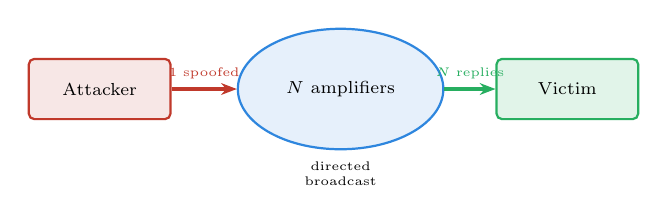
\begin{tikzpicture}[scale=0.9,transform shape]
        \node[att]    (a) at (0,0) {Attacker};
        \node[draw,thick,ellipse,fill=ampc!12,draw=ampc,
              minimum width=2.9cm,minimum height=1.7cm,font=\scriptsize,align=center]
              (c) at (3.4,0) {$N$ amplifiers};
        \node[vic]    (v) at (6.6,0) {Victim};
        \draw[flow,attc] (a) -- node[above,font=\tiny]{1 spoofed} (c);
        \draw[flow,vicc] (c) -- node[above,font=\tiny]{$N$ replies} (v);
        \node[font=\tiny,align=center] at (3.4,-1.2){directed\\broadcast};
      \end{tikzpicture}
      \vspace{4pt}
      \footnotesize The victim absorbs $N\times$ the attacker's traffic; the
      attacker's address never appears.
    \end{column}
  \end{columns}
\end{frame}

% =====================================================================
\begin{frame}{Two attacks, one root cause}
  \centering
  \begin{tabular}{@{}lll@{}}
    \toprule
     & \textbf{Smurf} & \textbf{Fraggle} \\
    \midrule
    Layer-4 protocol      & ICMP echo (type 8) & UDP echo (port 7) \\
    Amplifier answers because & it replies to broadcast ping & it runs an echo service \\
    Spoofed source        & victim & victim \\
    Destination           & subnet broadcast & subnet broadcast \\
    Measured factor ($N{=}3$) & \textbf{3.00} & \textbf{3.00} \\
    \bottomrule
  \end{tabular}

  \vspace{6pt}
  \begin{beamercolorbox}[wd=0.9\textwidth,center,rounded=true,shadow=false]{palette primary}
    \small\textbf{Thesis:} the \emph{misconfiguration}, not the protocol, is the vulnerability.
  \end{beamercolorbox}
\end{frame}

% =====================================================================
\section{Lab setup}
\begin{frame}{Isolated lab topology — 6 namespaces, 2 bridges, 1 router}
  \centering
  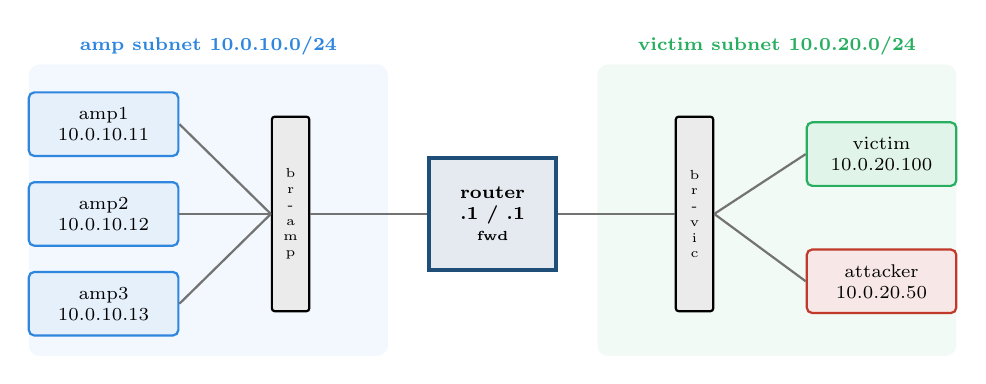
\begin{tikzpicture}[scale=0.95,transform shape]
    % subnet backdrops
    \begin{scope}[on background layer]
      \fill[ampc!6,rounded corners] (-6.2,-1.9) rectangle (-1.4,2.0);
      \fill[vicc!6,rounded corners] ( 1.4,-1.9) rectangle ( 6.2,2.0);
    \end{scope}
    \node[font=\scriptsize\bfseries,ampc] at (-3.8,2.25) {amp subnet 10.0.10.0/24};
    \node[font=\scriptsize\bfseries,vicc] at ( 3.8,2.25) {victim subnet 10.0.20.0/24};

    % amplifiers
    \node[amp] (a1) at (-5.2, 1.2) {amp1\\10.0.10.11};
    \node[amp] (a2) at (-5.2, 0.0) {amp2\\10.0.10.12};
    \node[amp] (a3) at (-5.2,-1.2) {amp3\\10.0.10.13};
    % bridges
    \node[bridge] (bra) at (-2.7,0) {b\\r\\-\\a\\m\\p};
    \node[bridge] (brv) at ( 2.7,0) {b\\r\\-\\v\\i\\c};
    % router
    \node[router] (r) at (0,0) {router\\\scriptsize .1 / .1\\\tiny fwd};
    % victim side
    \node[vic] (v)  at (5.2, 0.8) {victim\\10.0.20.100};
    \node[att] (at) at (5.2,-0.9) {attacker\\10.0.20.50};

    % links
    \foreach \n in {a1,a2,a3} \draw[link] (\n.east) -- (bra.west);
    \draw[link] (bra.east) -- (r.west);
    \draw[link] (r.east)   -- (brv.west);
    \draw[link] (v.west)   -- (brv.east);
    \draw[link] (at.west)  -- (brv.east);
  \end{tikzpicture}

  \vspace{2pt}
  \footnotesize Both bridges live \emph{inside} the router namespace; the only path
  between subnets is the router. Nothing is bridged to a real NIC $\Rightarrow$ no
  internet / campus route.
\end{frame}

% =====================================================================
\begin{frame}{The attack packet path}
  \centering
  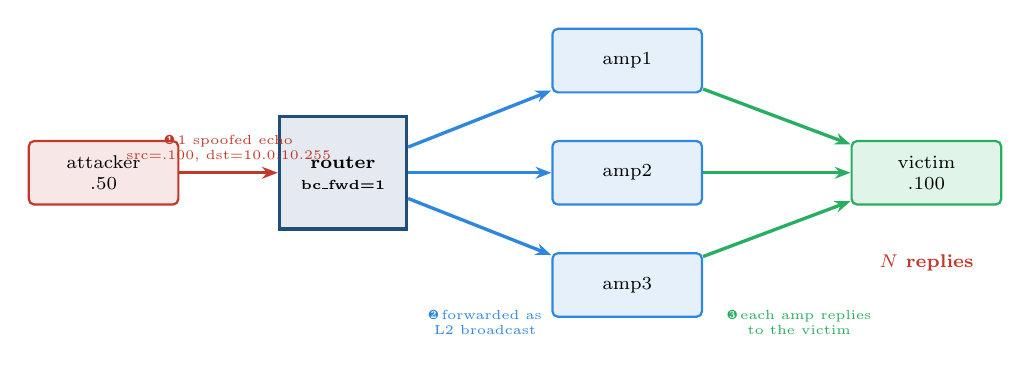
\begin{tikzpicture}[scale=0.95,transform shape]
    \node[att]    (at) at (-5.4,0)   {attacker\\.50};
    \node[router] (r)  at (-2.2,0)   {router\\\tiny bc\_fwd=1};
    \node[amp] (a1) at (1.6, 1.5) {amp1};
    \node[amp] (a2) at (1.6, 0.0) {amp2};
    \node[amp] (a3) at (1.6,-1.5) {amp3};
    \node[vic]    (v)  at (5.6,0)    {victim\\.100};

    \draw[flow,attc] (at) -- node[above,font=\tiny,align=center]
        {\ding{182}\,1 spoofed echo\\src=.100, dst=10.0.10.255} (r);
    \foreach \n in {a1,a2,a3}
        \draw[flow,ampc] (r) -- node[pos=0.6,font=\tiny]{} (\n);
    \node[ampc,font=\tiny,align=center] at (-0.3,-2.0){\ding{183}\,forwarded as\\L2 broadcast};
    \foreach \n in {a1,a2,a3}
        \draw[flow,vicc] (\n) -- (v);
    \node[vicc,font=\tiny,align=center] at (3.9,-2.0){\ding{184}\,each amp replies\\to the victim};
    \node[font=\scriptsize\bfseries,attc] at (5.6,-1.2){$N$ replies};
  \end{tikzpicture}
  \vspace{4pt}
  \footnotesize \textbf{Result:} 100 spoofed requests $\rightarrow$ 300 replies at the
  victim (3 amplifiers). The attacker (.50) never appears in the flood.
\end{frame}

% =====================================================================
\begin{frame}[fragile]{Hand-crafted senders — no \code{hping}/\code{nping}/\code{scapy}}
  \begin{columns}[T]
    \begin{column}{0.5\textwidth}
      \small
      Every IP / ICMP / UDP header field and \textbf{every checksum} is built by hand
      over a raw socket:
      \begin{itemize}\small
        \item \code{smurf.py} / \code{smurf.c} — ICMP Smurf
        \item \code{fraggle.py} / \code{fraggle.c} — UDP Fraggle
        \item \code{udp\_echo.py} — the amplifier's echo service
      \end{itemize}
      \footnotesize
      Raw \code{AF\_INET / SOCK\_RAW / IPPROTO\_RAW} + \code{IP\_HDRINCL}; the UDP
      checksum also covers the 12-byte pseudo-header (RFC 768).
    \end{column}
    \begin{column}{0.5\textwidth}
\begin{verbatim}
def checksum(data):     # RFC 1071
    if len(data)%2: data+=b"\x00"
    t=0
    for i in range(0,len(data),2):
        t+=(data[i]<<8)|data[i+1]
    t=(t>>16)+(t&0xffff); t+=t>>16
    return (~t)&0xffff

s=socket(AF_INET,SOCK_RAW,IPPROTO_RAW)
s.setsockopt(IPPROTO_IP,IP_HDRINCL,1)
s.sendto(ip_hdr+icmp, (bcast,0))
\end{verbatim}
    \end{column}
  \end{columns}
\end{frame}

% =====================================================================
\begin{frame}{Deliberately vulnerable configuration (lab-only, torn down after)}
  \centering
  \small
  \begin{tabular}{@{}lllc@{}}
    \toprule
    \textbf{Where} & \textbf{Setting / state} & \textbf{Vulnerable} & \textbf{Secure} \\
    \midrule
    router  & \code{net.ipv4.ip\_forward}                    & 1 & 1 (routing) \\
    router  & \code{net.ipv4.conf.*.bc\_forwarding}          & \textcolor{attc}{\textbf{1}} & 0 \\
    router  & \code{net.ipv4.conf.*.rp\_filter}              & 0 & (varies) \\
    amp1--N & \code{net.ipv4.icmp\_echo\_ignore\_broadcasts} & \textcolor{attc}{\textbf{0}} & 1 \\
    amp1--N & UDP echo service (\code{udp\_echo.py})          & \textcolor{attc}{\textbf{on}} & off \\
    edge    & IP source guard on attacker port               & \textcolor{attc}{\textbf{absent}} & present \\
    \bottomrule
  \end{tabular}

  \vspace{6pt}
  \footnotesize All vulnerable state lives only inside the namespaces and is removed by
  \code{teardown\_lab.sh}.
\end{frame}

% =====================================================================
\section{Measurement \& results}
\begin{frame}{Measurement methodology — counted at the victim, two independent ways}
  \begin{columns}[T]
    \begin{column}{0.5\textwidth}
      \textbf{ICMP (Smurf)}
      \begin{itemize}\small
        \item \code{tcpdump} pcap of echo-replies
        \item kernel counter \code{IcmpMsg InType0}
        \item cross-check \code{Icmp InEchoReps}
      \end{itemize}
      \textbf{UDP (Fraggle)}
      \begin{itemize}\small
        \item \code{tcpdump} pcap of replies to the spoofed source port
        \item kernel counter \code{Udp NoPorts}
              \footnotesize (victim isn't listening $\Rightarrow$ each reply counts here)
      \end{itemize}
    \end{column}
    \begin{column}{0.5\textwidth}
      \begin{block}{Amplification factor}
        \centering\small
        $\dfrac{\text{replies received at victim}}{\text{requests sent by attacker}}$
      \end{block}
      \footnotesize
      All three counters agree exactly. Every run is appended to
      \code{results/summary.tsv} and reproduced by \code{run\_all.sh}
      (100 requests/run at 50\,pps).
    \end{column}
  \end{columns}
\end{frame}

% =====================================================================
\begin{frame}{Results — the attack works, both protocols, both senders}
  \centering
  \small
  \begin{tabular}{@{}llccc@{}}
    \toprule
    \textbf{Scenario} & \textbf{Sender} & \textbf{Sent} & \textbf{Replies} & \textbf{Factor}\\
    \midrule
    Vulnerable & \code{smurf.py}   & 100 & 300 & \textbf{3.00}\\
    Vulnerable & \code{smurf.c}    & 100 & 300 & \textbf{3.00}\\
    Vulnerable & \code{fraggle.py} & 100 & 300 & \textbf{3.00}\\
    Vulnerable & \code{fraggle.c}  & 100 & 300 & \textbf{3.00}\\
    Revert $\rightarrow$ recheck & \code{smurf.py} & 100 & 300 & \textbf{3.00}\\
    \bottomrule
  \end{tabular}

  \vspace{6pt}
  \footnotesize Both hand-written senders (Python \& C) give identical results —
  confirming the by-hand headers and all three checksums (IP, ICMP, UDP pseudo-header).
\end{frame}

% =====================================================================
\section{Defenses}
\begin{frame}{Layered defenses — which layer stops which attack}
  \centering
  \small
  \begin{tabular}{@{}p{4.7cm}p{3.2cm}cc@{}}
    \toprule
    \textbf{Defense (applied alone)} & \textbf{Layer} & \textbf{Smurf} & \textbf{Fraggle}\\
    \midrule
    \code{bc\_forwarding=0} (router) & routing & \yes & \yes\\
    \code{icmp\_echo\_ignore\_broadcasts=1} & ICMP host & \yes & \no\\
    stop UDP echo service (amps) & UDP host & \no & \yes\\
    edge IP source guard (nft bridge) & source validation & \yes & \yes\\
    \bottomrule
  \end{tabular}

  \vspace{5pt}
  \begin{itemize}\footnotesize
    \item \textbf{Router fix} and \textbf{edge source guard} are \emph{universal} — they
          attack the root cause (the forwarded broadcast / the spoof itself).
    \item Per-host fixes are \emph{protocol-specific}: silencing broadcast ping does
          nothing to a UDP Fraggle, and vice-versa.
    \item Source guard is \emph{per-port}: plain subnet uRPF cannot catch a spoof of an
          address that is itself valid on the victim subnet.
  \end{itemize}
\end{frame}

% =====================================================================
\begin{frame}{Defense matrix — measured factor per defense}
  \centering
  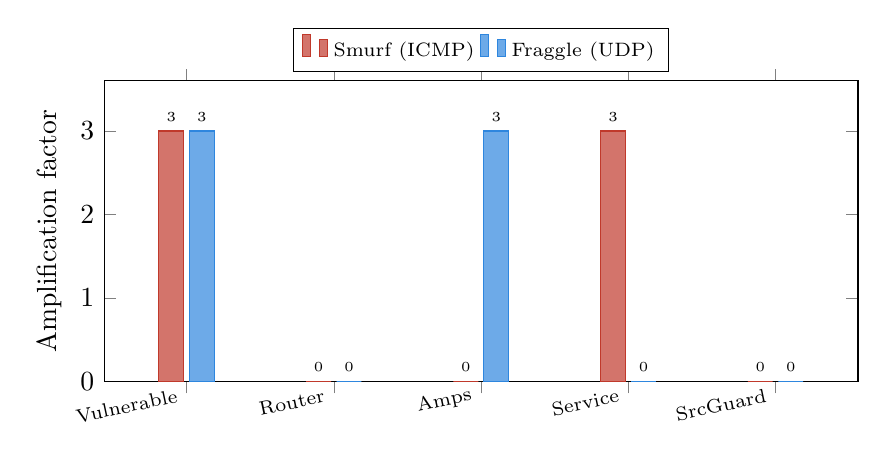
\begin{tikzpicture}
    \begin{axis}[
        ybar, bar width=9pt,
        width=0.92\linewidth, height=5.4cm,
        ymin=0, ymax=3.6, ylabel={Amplification factor},
        symbolic x coords={Vulnerable,Router,Amps,Service,SrcGuard},
        xtick=data, x tick label style={font=\scriptsize,rotate=12,anchor=east},
        enlarge x limits=0.14,
        nodes near coords, nodes near coords style={font=\tiny},
        legend style={at={(0.5,1.03)},anchor=south,legend columns=-1,font=\scriptsize},
      ]
      \addplot[fill=attc!70,draw=attc]  coordinates
        {(Vulnerable,3)(Router,0)(Amps,0)(Service,3)(SrcGuard,0)};
      \addplot[fill=ampc!70,draw=ampc]  coordinates
        {(Vulnerable,3)(Router,0)(Amps,3)(Service,0)(SrcGuard,0)};
      \legend{Smurf (ICMP), Fraggle (UDP)}
    \end{axis}
  \end{tikzpicture}

  \footnotesize The two protocol-specific fixes each leave the \emph{other} attack fully
  amplifying (factor 3) — the visual proof of the thesis.
\end{frame}

% =====================================================================
\section{Scaling}
\begin{frame}{Amplification scales with the number of amplifiers}
  \begin{columns}[c]
    \begin{column}{0.6\textwidth}
      \centering
      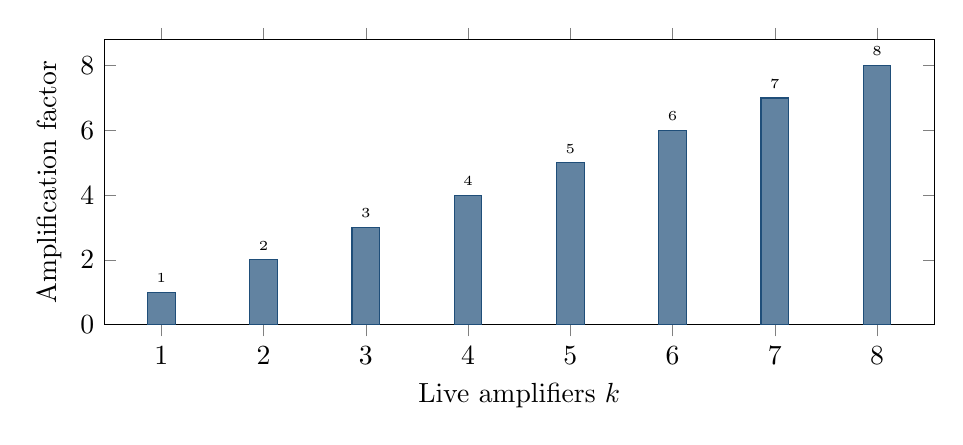
\begin{tikzpicture}
        \begin{axis}[
            ybar, bar width=10pt,
            width=\linewidth, height=5.2cm,
            xlabel={Live amplifiers $k$}, ylabel={Amplification factor},
            xtick={1,2,3,4,5,6,7,8}, ymin=0, ymax=8.8,
            nodes near coords, nodes near coords style={font=\tiny},
            enlarge x limits=0.08,
          ]
          \addplot[fill=primary!70,draw=primary] coordinates
            {(1,1)(2,2)(3,3)(4,4)(5,5)(6,6)(7,7)(8,8)};
        \end{axis}
      \end{tikzpicture}
    \end{column}
    \begin{column}{0.4\textwidth}
      \small
      \code{scale\_test.sh} enables $k$ of the amplifiers and fires the identical attack.
      \[ \text{factor}(k)=k \]
      \footnotesize
      Verified $k=1\ldots8$ via the overridable \code{AMP\_COUNT}. A real /24 with
      hundreds of responders yields a three-order-of-magnitude multiplier from a single
      spoofed packet.
    \end{column}
  \end{columns}
\end{frame}

% =====================================================================
\begin{frame}[fragile]{Packet-path proof — from the live captures}
  \textbf{Smurf (ICMP):} one broadcast request, three replies to the victim
\begin{verbatim}
router br-vic (in):  10.0.20.50 > 10.0.10.255: ICMP echo request
router br-amp (out): 10.0.20.50 > 10.0.10.255: ICMP echo request   <- forwarded
amp1 eth0:  .. > ff:ff:ff:ff:ff:ff  10.0.20.50 > 10.0.10.255  echo request
router br-vic (in):  10.0.10.11 > 10.0.20.50: ICMP echo reply
                     10.0.10.12 > 10.0.20.50: ICMP echo reply
                     10.0.10.13 > 10.0.20.50: ICMP echo reply       <- 3 replies
\end{verbatim}
  \textbf{Fraggle (UDP):} identical amplification over UDP echo (port 7)
\begin{verbatim}
10.0.10.11.7 > 10.0.20.100.40000: UDP, length 7
10.0.10.13.7 > 10.0.20.100.40000: UDP, length 7
10.0.10.12.7 > 10.0.20.100.40000: UDP, length 7      <- one reply per amp
\end{verbatim}
\end{frame}

% =====================================================================
\section{Tooling \& safety}
\begin{frame}{Tooling \& reproducibility}
  \begin{columns}[T]
    \begin{column}{0.54\textwidth}
      \small\textbf{One command reproduces everything:}
      \begin{itemize}\small
        \item \code{setup\_lab.sh} — build namespaces/bridges + vulnerable config
        \item \code{run\_all.sh} — full attack $\times$ defense matrix
        \item \code{scale\_test.sh} — factor vs. amplifier count
        \item \code{defend.sh} — \code{router|amps|service|spoofguard|all|revert}
        \item \code{measure.sh} \code{--proto icmp|udp}
        \item \code{preflight.sh} — kernel capability check
        \item \code{teardown\_lab.sh} — remove everything
      \end{itemize}
    \end{column}
    \begin{column}{0.46\textwidth}
      \small\textbf{Platform / framework}
      \begin{itemize}\small
        \item Linux network namespaces, \code{veth}, bridges (\code{iproute2})
        \item \code{nftables} bridge family (source guard)
        \item C (\code{gcc}) + Python 3 stdlib \code{socket}
        \item Bash orchestration; \code{/proc/net/snmp} + \code{tcpdump}
        \item \textbf{No framework, no attack libraries}
      \end{itemize}
      \footnotesize\textbf{Needs kernel:} \code{bridge} + \code{bc\_forwarding}
      ($\geq$ 5.1). Default WSL2 kernels may lack these — \code{preflight.sh} verifies.
    \end{column}
  \end{columns}
\end{frame}

% =====================================================================
\begin{frame}{Safety invariants \& conclusion}
  \begin{block}{Safety}
    \small
    All six namespaces are internal — nothing bridged to a real NIC $\Rightarrow$ no
    internet / campus route. Vulnerable sysctls and responders exist only inside
    namespaces and are torn down. Low, instrumented rate — we demonstrate the
    \emph{multiplier}, not throughput.
  \end{block}
  \begin{block}{Key takeaways}
    \begin{itemize}\small
      \item One spoofed packet $\rightarrow$ $N$ replies; \textbf{factor $=N$}, measured
            and reproducible (3.00 at $N{=}3$; linear to $k{=}8$).
      \item Smurf and Fraggle amplify identically — \textbf{the misconfiguration, not the
            protocol, is the bug}.
      \item Disabling directed-broadcast forwarding (or validating the source at the edge)
            stops \emph{both}; per-host fixes stop only one.
      \item Everything hand-built on raw sockets; fully isolated; one-command reproducible.
    \end{itemize}
  \end{block}
  \centering\vspace{2pt}
  {\small\textcolor{primary}{\textbf{Thank you.}}\quad Questions?}
\end{frame}

\end{document}
